\documentclass[output=paper]{langsci/langscibook}
\ChapterDOI{10.5281/zenodo.3744501}
\author{Christopher Lucas\affiliation{SOAS University of London}\lastand Stefano Manfredi\affiliation{CNRS, SeDyL}}
\title{Introduction}
% \keywords{}
\abstract{This introductory chapter gives an overview of the aims, scope, and approach of the volume, while also providing a thematic bibliography of the most significant previous literature on Arabic and contact-induced change.}
\maketitle

\begin{document}\label{introintro}

\section{Rationale}
With its lengthy written history, wide and well-studied dialectal variation, and involvement in numerous heterogeneous contact situations, the \ili{Arabic} language has an enormous contribution to make to our understanding of how language contact can lead to change. Until now, however, most of what is known about the diverse outcomes of contacts between \ili{Arabic} and other languages has remained inaccessible to non-specialists. There are brief summary sketches \citep{Versteegh2001article,Versteegh2010,Thomason2011,Manfredi2018}, as well as a recent collection of articles on a range of issues connected with \ili{Arabic} and language contact in general \citep{ManfrediTosco2018}, but no larger synthesis of the kind that is available, for example, for Amazonian languages \citep{Aikhenvald2002}.

\ili{Arabic} has thus played little part in work to date on contact-induced change that is crosslinguistic in
scope (though see \citealt{Matras2009,Trudgill2011} for partial exceptions). By providing the community of general and historical linguists with the present collaborative synthesis of expertise on \ili{Arabic} and contact-induced change, we hope to help rectify this situation. The work consists of twenty-nine chapters by leading authorities in their fields, and is divided into three Parts: overviews of contact-induced change in individual \ili{Arabic} varieties (Part I); overviews of the outcomes of contact with \ili{Arabic} in other languages (Part II); and overviews of various types of changes across \ili{Arabic} varieties, in which contact has played a significant role (Part III). Chapters in each of the three Parts follow the fixed broad outlines detailed below in §\ref{introstructure}, in order to maximize coherence and ease of reference. All authors have also been encouraged a) to ensure their chapters contain a rich set of (uniformly glossed and transcribed) linguistic data, including original data where appropriate, and b) to provide as much sociohistorical data as possible on the speech communities involved, framed where possible with reference to Van Coetsem’s (\citeyear{VanCoetsem1988,VanCoetsem2000}) distinction between changes due to borrowing (by agents dominant in the {recipient language} ({RL})) and {imposition} (by agents dominant in the {source language} ({SL}); see §\ref{introvc} for further details). These features are aimed at ensuring that the data presented in the volume can be productively drawn upon by scholars and students of linguistics who are not specialists in
\ili{Arabic} linguistics, and especially those working on the mechanisms, typology, outcomes, and theory of contact-induced change cross-linguistically.


The rest of this introductory chapter is structured as follows. We begin by providing a thematic bibliography of existing work on \ili{Arabic} and contact-induced change in §\ref{introexistingwork}. The overall scope of the present volume is then detailed in §\ref{introscope}. §\ref{introwherewhat} locates and classifies the different varieties of what is called ``\ili{Arabic}'' according to Jastrow's (\citeyear{Jastrow2002}) three geographic zones and Labov's (\citeyear{Labov2007}) concepts of {transmission} and {diffusion} in {language change}, while §\ref{intropartIoverview}--§\ref{intropartIIIoverview} provide an overview of the content of each of the three Parts into which the present volume is divided. In §\ref{introvc} we give details of Van Coetsem's (\citeyear{VanCoetsem1988,VanCoetsem2000}) framework, and in §\ref{introstructure} we outline the common structure and transcription and glossing conventions of the volume. This introductory chapter then finishes with §\ref{introthemes}, in which we discuss some of the challenges to Van Coetsem's framework posed by the data in this volume, how these challenges can be addressed, and how the data and analyses collected in the present work can be built on by others.


\section{Previous work}\label{introexistingwork}

As noted in §\ref{introintro}, there is a reasonably large existing literature {focusing} on specific aspects of \ili{Arabic} and contact-induced change. For reviews of much of this literature, readers are referred to the relevant chapters of the present volume. Here we simply list some key works for ease of reference in the following (non-comprehensive) bibliography, organized by linguistic variety.\pagebreak

\begin{itemize}[noitemsep,leftmargin=11pt]
\item[\adfhalfrightarrowhead]\ili{Old Arabic} and \ili{Middle Aramaic}: \citet{Retsö2011}, \citet{Weninger2011Aramaic}, \citet{Owens2016Aramaic}.

\item[\adfhalfrightarrowhead]\ili{Arabic} and \ili{Neo-Aramaic}:
\citet{ArnoldBehnstedt1993}, \citet{Arnold2007}, Coghill (\citeyear{Coghill2010,Coghill2012,Coghill2015}), \citet{Jastrow2015}.

\item[\adfhalfrightarrowhead]\ili{Arabic} and \ili{Hebrew}:
\citet{Blau1981}, \citet{Yoda2013}, \citet{Horesh2015}.

\item[\adfhalfrightarrowhead]\ili{Arabic} and (Modern) \ili{South Arabian} languages: \citet{Diem1979}, \citet{Lonnet2011}, \citet{Zammit2011}, \citet{Watson2018}.

\item[\adfhalfrightarrowhead]\ili{Arabic} and \ili{Indo-Iranian} languages: \citet{Tsabolov1994}, \citet{Matras2007Domari}, \citet{Asbaghi2011}, \citet{Gazsi2011}, \citet{WalAnonby2015}, \citet{Herin2018}.

\item[\adfhalfrightarrowhead]\ili{Arabic} and \ili{Turkish}: Procházka (\citeyear{Procházka2002Adana,Procházka2011Turkish}), \citet{Haig2014}, \citet{Taylan2017}, \citet{AkkusBenmamoun2018}.


\item[\adfhalfrightarrowhead]\ili{Arabic} and \ili{Berber}: Taine-Cheikh (\citeyear{Taine-Cheikh1997Zenaga,Taine-Cheikh2018quadri}), \citet{Brahimi2000}, \citet{Corriente2002}, \citet{LafkiouiBrugnatelli2008}, Kossmann
(\citeyear{Kossmann2009,Kossmann2010,Kossmann2013book}), \citet{ElAissati2011}, \citet{Lafkioui2013reinventing}, \citet{Souag2013book},  \citet{vanPuttenSouag2015}.

\item[\adfhalfrightarrowhead]\ili{Arabic} and (sub-)Saharan languages: \citet{Owens2000article,Owens2015}, \citet{Lafkioui2013book}, \citet{Souag2016sahara}.


\item[\adfhalfrightarrowhead]\ili{Arabic} and \ili{Latin}/\ili{Romance} languages: \citet{Brunot1949}, \citet{Benoliel1977}, Corriente (\citeyear{Corriente1978,Corriente1992book}), \citet{Talmoudi1986}, Heath (\citeyear{Heath1989,Heath2015}), \citet{Cifoletti1994}, \citet{Vicente2006}, \citet{Sayahi2014}.

\item[\adfhalfrightarrowhead]Contact influences on \ili{Classical} and \ili{Modern Standard} \ili{Arabic} (\ili{MSA}): \citet{Jeffrey2007} [1938], \citet{Blau1969}, \citet{Hebbo1984}.

\item[\adfhalfrightarrowhead]Contact influence in \ili{Mesopotamian} \ili{Arabic}: Masliyah (\citeyear{Masliyah1996,Masliyah1997}), \citet{MatrasShabibi2007}, \citet{ElZarkaZiagos2019}.

\item[\adfhalfrightarrowhead]Contact influence in \ili{Central Asian} \ili{Arabic}: \citet{Jastrow2005}, \citet{Ratcliffe2005}, \citet{Ingham2011afg}.

\item[\adfhalfrightarrowhead]Contact influence in \ili{Levantine} \ili{Arabic}: \citet{Barbot1961}, \citet{Neishtadt2015}.

\item[\adfhalfrightarrowhead]Contact influence in \ili{Cypriot Maronite} \ili{Arabic}: \citet{Newton1964}, \citet{Tsiapera1964}, Borg (\citeyear{Borg1997CMA,Borg2004}).

\item[\adfhalfrightarrowhead]Contact influence in \ili{Maltese}: \citet{colin1957}, \citet{Aquilina1958}, \citet{krier1976},  \citet{mifsudloanverbs}, \citet{brincat2011}, \citet{Souag2018berber}.

\item[\adfhalfrightarrowhead]\ili{Arabic} pidgins and creoles: \citet{Owens1985}, \citet{Miller1993}, \citet{Luffin2014}, \citet{Avram2017article}, \citet{Bizri2018}, \citet{Owens2018}.

\item[\adfhalfrightarrowhead]Contact between \ili{Arabic} dialects:  \citet{Gibson2002}, \citet{Miller2007}, \citet{CotterHoresh2015}, \citet{Leddy-Cecere2018}.

\end{itemize}

\section{Scope}\label{introscope}

\subsection{Where and what is Arabic?}\label{introwherewhat}

\ili{Arabic} is one of the most widely spoken languages in the world, and the first language of around 350 million speakers spread throughout the Middle East and North Africa. There are twenty-five sovereign states in which \ili{Arabic} is an official language. In addition, \ili{Arabic} is widely spoken as a lingua franca (i.e. vehicular language) for a range of communicative interactions between different linguistic communities in Asia and Africa. Following Jastrow (\citeyear{Jastrow2002}; see also \citealt{Watson2011dialectsoverview}; \citealt{Manfrediforthcoming}), the present-day \ili{Arabic}-speaking world can be broadly subdivided into three geographic zones (cf. Figure \ref{intromap}): Zone I covers the regions of the Arabian Peninsula where \ili{Arabic} was spoken before the beginning of the Islamic expansion in the seventh century; Zone II includes the Middle Eastern and North African areas into which \ili{Arabic} penetrated during the Islamic expansion, and where it is today spoken as a majority language; and Zone III encompasses isolated regions where \ili{Arabic} is spoken today by minority bilingual communities (see also \citealt{Owens2000editor}). Further to this, following successive waves of mass emigration in recent centuries, \ili{Arabic} is also spoken as a heritage language by diasporic communities around the world (\citealt{Rouchdy_arabic_1992,BoumansdeRuiter2002}; D’Anna, this volume).\ia{D'Anna, Luca@D'Anna, Luca} Against the backdrop of this complex geo-historical distribution, the question that arises is what unites all the varieties that fall under the glottonym ``\ili{Arabic}'' and, more generally, what should count as \ili{Arabic} from a linguistic point of view?

\begin{figure}
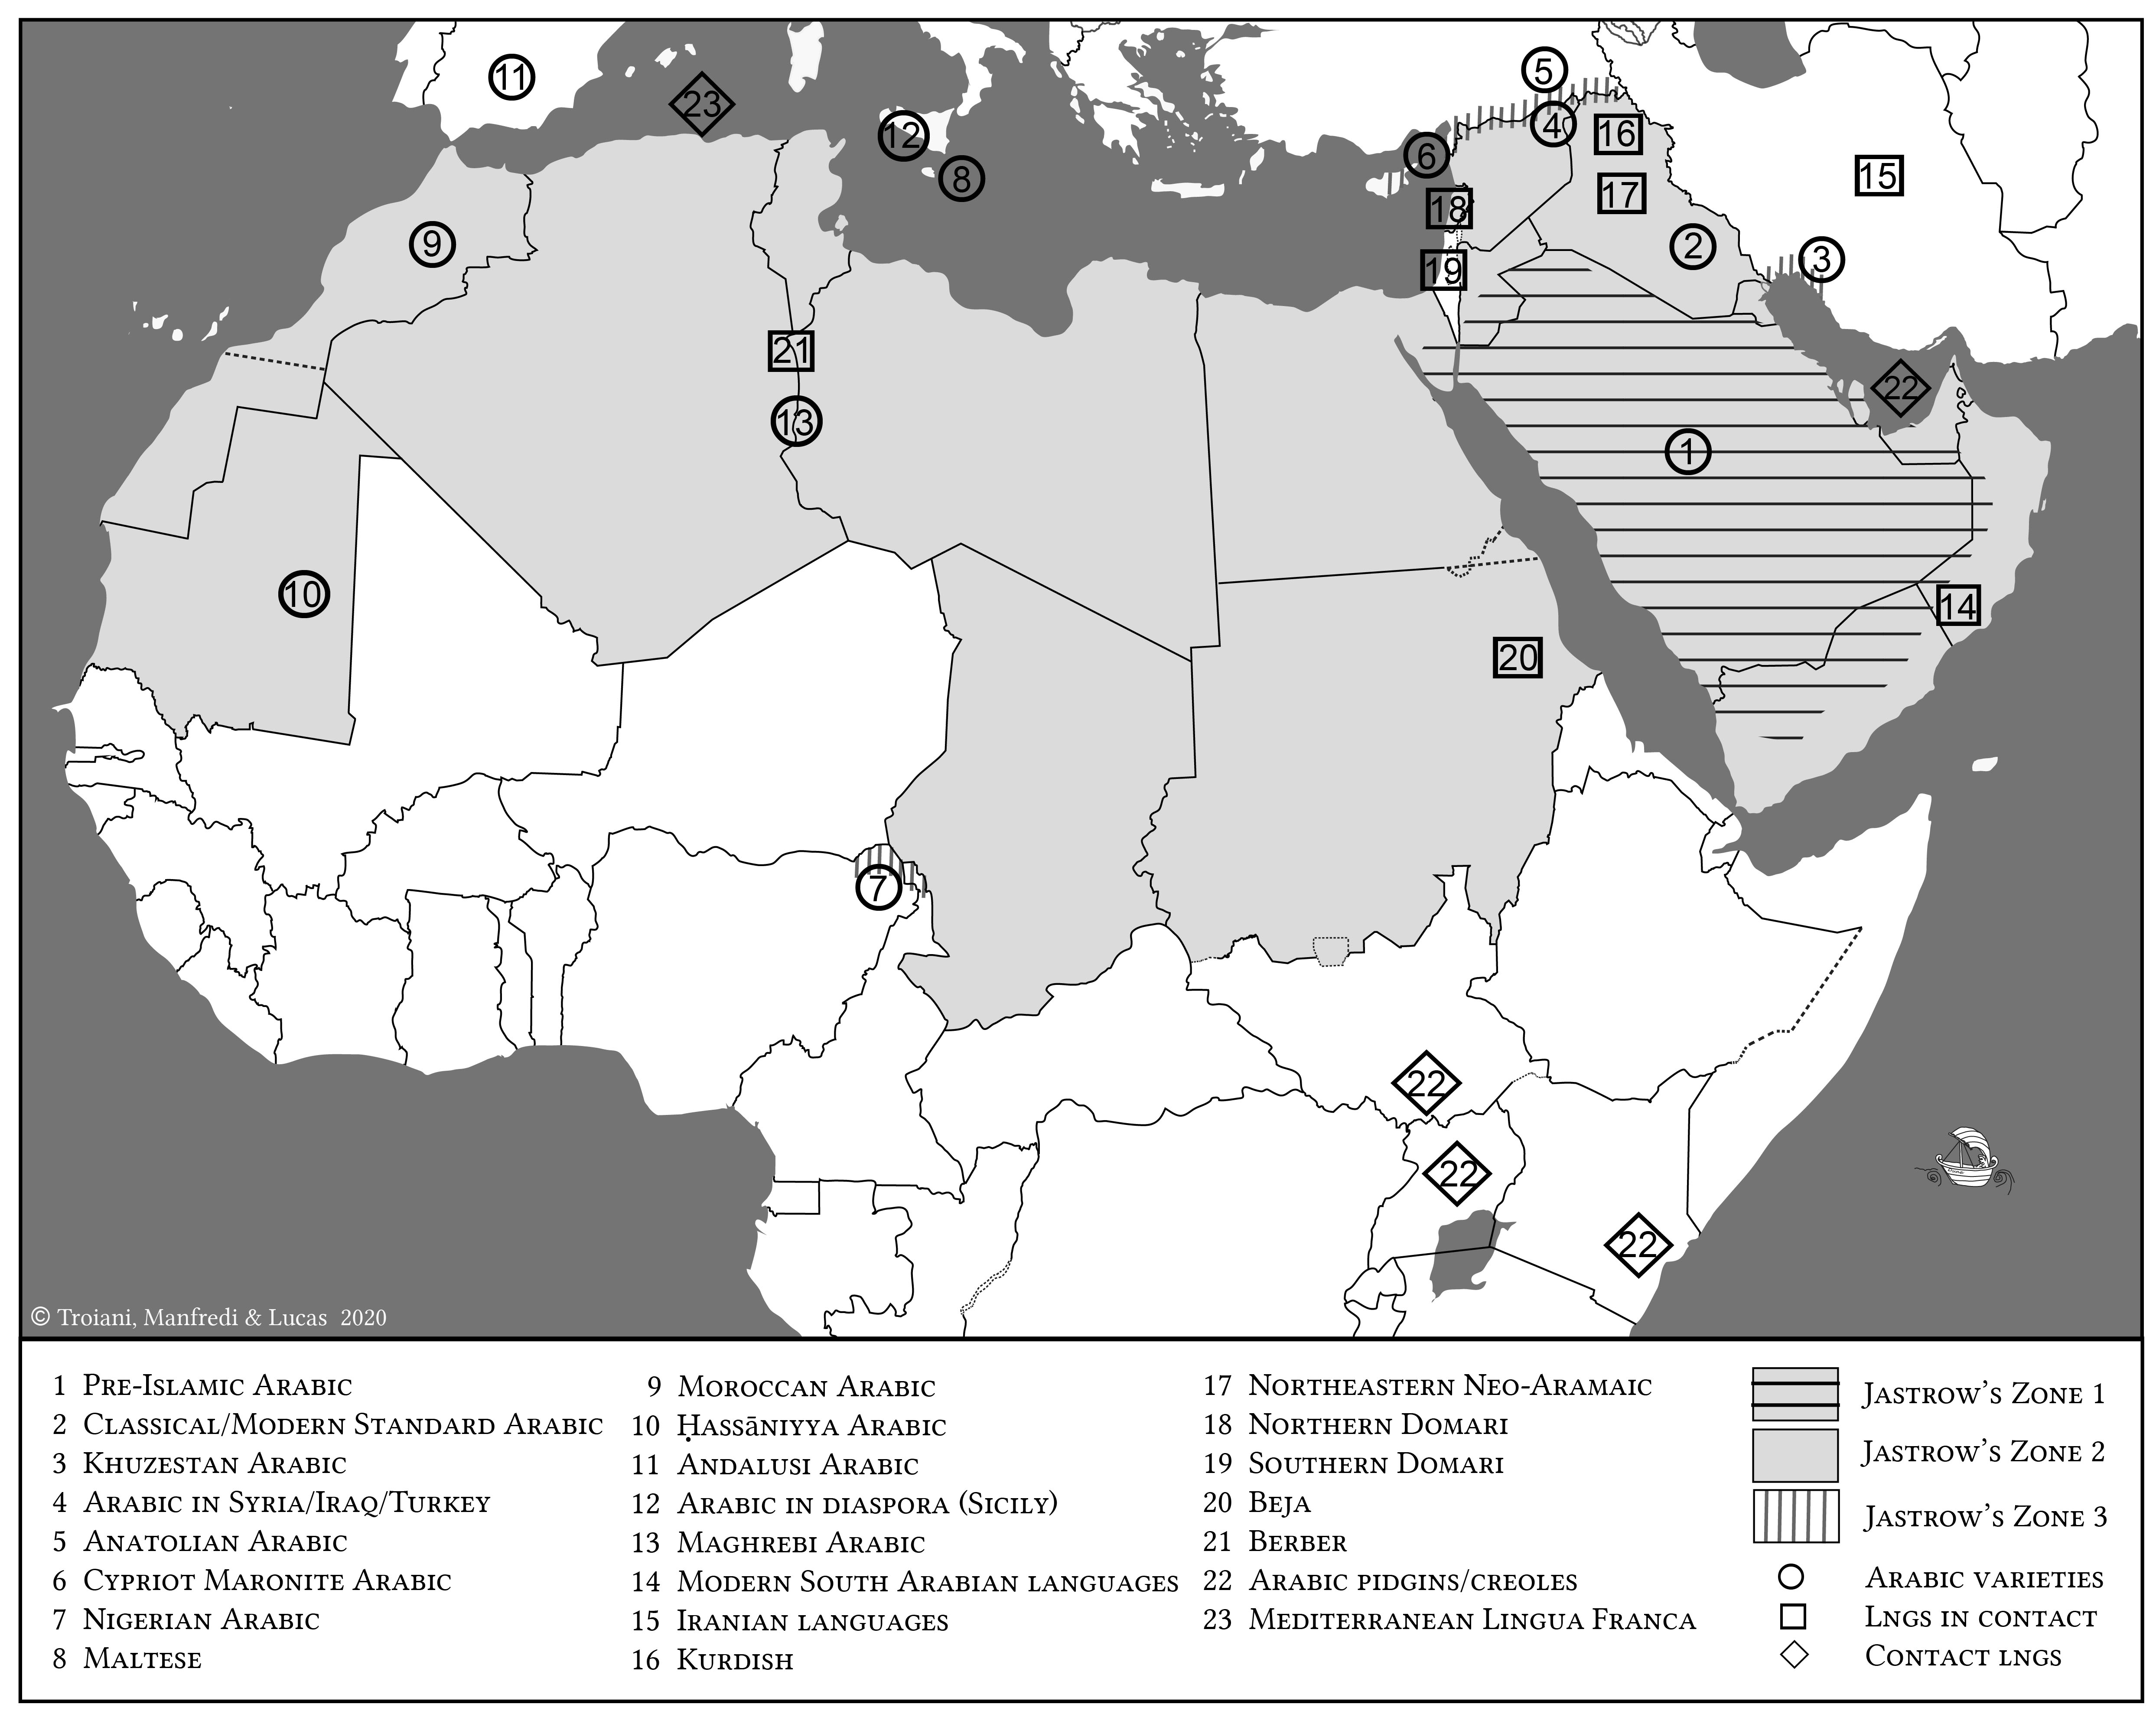
\includegraphics[width=\textwidth]{figures/intromap.jpg}
\caption{Approximate distribution of languages and Arabic varieties discussed in this volume}
\label{intromap}
\end{figure}

After all, the term ``\ili{Arabic}'' encompasses a great deal of internal variety, whose origins can be traced back to both internally and externally motivated (i.e. con\-tact-induced) changes. One way of understanding these different patterns of {language change} is through Labov's (\citeyear{Labov2007}) distinction between \textsc{transmission} and \textsc{diffusion}. If {transmission} refers to change through an unbroken sequence of first-language acquisition (\citealt{Labov2007}: 346), {diffusion} rather implies the {transfer} of features across languages via language/{dialect contact} (\citealt{Labov2007}: 347). Change through {transmission} is said to be regular because it is incremented by young native speakers, whereas {diffusion} is thought to be more irregular and unpredictable because it is typically produced by adult bilingual speakers. Both mechanisms contribute to long-term {language change} even though, according to Labov, {transmission} is the foremost mechanism by which linguistic diversity is produced and maintained. In a recent study, \citet{Owens2018} tests the generality of the Labovian distinction between {transmission} and {diffusion} against the complex linguistic and sociohistorical patchwork of \ili{Arabic}. He concludes that change through {diffusion} cannot be said to be more irregular than change via {transmission} and that, other than for \ili{Arabic}-based creoles (see Avram, this volume),\ia{Avram, Andrei A.@Avram, Andrei A.} there are no clear-cut criteria for distinguishing the two mechanisms of {language change}. The reason for this is that most of the linguistic varieties that are commonly referred to under the heading of ``\ili{Arabic}'' are the result of a longstanding series of multi-causal changes encompassing both internal drift and {convergence}, as well as contact-induced change via {diffusion}. What we do not see, however, in any of the varieties usually referred to as \ili{Arabic}, are the atypical kinds of changes produced by the disruption of language {transmission} as observed in {pidgin} and {creole} languages (but see below). Thus Part I of this volume primarily (but not exclusively) deals with contact-induced change in spoken varieties of \ili{Arabic} that have gone through an unbroken chain of language {transmission}, the so-called ``\ili{Arabic} dialects''.


\subsection{Overview of Part I: Contact-induced change in varieties of Arabic}\label{intropartIoverview}

The survey chapters in Part I of this volume offer an extensive overview of contact-induced change in first \ili{Eastern} (\textit{mašriqī}) and then \ili{Western} (\textit{maɣribī}) \ili{Arabic} dialects (to use the terminology of the traditional geographical classification of modern \ili{Arabic} dialects; cf. \citealt{Palva2009}; Benkato, this volume)\ia{Benkato, Adam@Benkato, Adam}. The majority of chapters dealing with types of Eastern Arabic describe varieties spoken by bilingual minorities affected to different degrees by {language shift} towards local dominant languages. For instance, the \ili{Arabic}-speaking Maronite community of {Kormakiti} is involved in an asymmetric pattern of {bilingualism} resulting in a gradual and inexorable {language shift} towards \ili{Cypriot Greek} (Walter, this volume).\ia{Walter, Mary Ann@Walter, Mary Ann} In contrast, speakers of \ili{Nigerian} \ili{Arabic} (Owens, this volume),\ia{Owens, Jonathan@Owens, Jonathan} despite considerable proficiency in \ili{Kanuri} and/or \ili{Hausa}, maintain {transmission} of their ancestral language to the younger generations. As far as it is possible to tell, a similar situation holds for the \ili{Mesopotamian} dialects of {Anatolia} (Akkuş, this volume)\ia{Akkuş, Faruk@Akkuş, Faruk} and \ili{Khuzestan} (Leitner, this volume),\ia{Leitner, Bettina@Leitner, Bettina} which are in intense contact with \ili{Turkish} and \ili{Persian} respectively (among other languages), but without (yet) showing signs of definitive {language shift}. Procházka (this volume),\ia{Procházka, Stephan@Procházka, Stephan} on the other hand, describes the effects of contact-induced change in a continuum of \ili{Eastern} \ili{Arabic} dialects dispersed across Lebanon, Syria, Iraq, and southern Turkey. In this broader geographical context, \ili{Arabic} represents the main vernacular language, affected to different degrees by long-term bi- or multilingualism with \ili{Aramaic}, \ili{Kurdish}, and \ili{Turkish}.

As far as \ili{Western Arabic} dialects are concerned, Benkato (this volume)\ia{Benkato, Adam@Benkato, Adam} describes a history of contact-induced change in different \ili{Maghrebi} dialects from the beginning of the {Arabization} of North Africa until the {colonial} period. Four further chapters then take a closer look at contact-induced changes in specific varieties of \ili{Western} \ili{Arabic}. Heath (this volume)\ia{Heath, Jeffrey@Heath, Jeffrey} covers \ili{Moroccan}, while Taine-Cheikh (this volume)\ia{Taine-Cheikh, Catherine@Taine-Cheikh, Catherine} covers \ili{Ḥassāniyya} -- two majority varieties of \ili{Arabic} historically affected by contact with \ili{Berber} and \ili{Romance} languages. Lucas \& Čéplö (this volume)\ia{Lucas, Christopher@Lucas, Christopher}\ia{Čéplö, Slavomír@Čéplö, Slavomír} then provide an overview of contact-induced change in \ili{Maltese} -- a variety which is no longer usually considered to be a subtype of ``\ili{Arabic}'', but which, as Lucas \& Čéplö show, is nevertheless historically part of the \ili{Western} group of \ili{Arabic} dialects. Indeed, despite the far-reaching lexical and grammatical effects of contact with Italo-\ili{Romance} and \ili{English}, \ili{Maltese} remains largely a product of {transmission} in the Labovian sense. We would not therefore classify it as a contact (i.e. mixed) language (cf. \citealt{stolz2003} and see further below). Lastly, D’Anna (this volume)\ia{D'Anna, Luca@D'Anna, Luca} offers a linguistic account of different varieties of \ili{Arabic} in diasporic settings, with particular focus on the \ili{Tunisian} community of {Mazara del Vallo} in {Sicily}. Unlike the \ili{Western} varieties described in the aforementioned chapters, in this latter context \ili{Arabic} is involved in an unbalanced contact situation, resulting in moderate {language shift} towards \ili{Sicilian} and \ili{Italian}.


As well as the aforementioned spoken varieties of \ili{Arabic}, Part I of the volume also includes three chapters analysing the outputs of language contact in different varieties of written \ili{Arabic}. First of all, Al-Jallad (this volume)\ia{Al-Jallad, Ahmad@Al-Jallad, Ahmad} describes a number of likely instances of contact-induced change in pre-Islamic \ili{Arabic} documentary sources (primarily inscriptional), and postulates the existence of different patterns of {bilingualism} between \ili{Arabic} and \ili{Akkadian}, \ili{Aramaic}, \ili{Old South Arabian}, and \ili{Greek} (among other languages). Van Putten (this volume)\ia{van Putten, Marijn@van Putten, Marijn} then focuses on contact influences on the later \ili{Classical} and \ili{MSA}, examining both early influences from \ili{Aramaic}, \ili{Greek}, \ili{Persian}, \ili{Ethio-Semitic} and \ili{Old South Arabian}, as well as later influence from \ili{Ottoman} {Turkish} and twentieth-century journalism in European languages. Since these written varieties of \ili{Arabic} are rather artificial constructs, van Putten also examines the influence of the native \ili{Arabic} dialects of the authors of texts in \ili{Classical} \ili{Arabic} and \ili{MSA}. The third and final written \ili{Arabic} variety analysed in this volume is \ili{Andalusi} \ili{Arabic}. Attested as a form of Middle \ili{Arabic} (\citealt{Lentin2011Middle}) between the tenth and seventeenth centuries, \ili{Andalusi} \ili{Arabic} displays significant grammatical and lexical input from both \ili{Romance} and \ili{Berber} languages (Vicente, this volume).\ia{Vicente, Ángeles@Vicente, Ángeles} As evidence for the \ili{Arabic} varieties described in these three chapters is exclusively written, they cannot be treated in the same manner as spoken varieties which emerged in a context of first language acquisition. They are, however, representative of a longstanding and uninterrupted written tradition that goes back to the pre-Islamic period, and that has always been in a multi-faceted relationship of mutual influence with different varieties of spoken \ili{Arabic}. In this sense, despite their rather artificial nature, written varieties of \ili{Arabic} may also be considered the product of language {transmission}.


In the final chapter of Part I, on the other hand, Avram (this volume)\ia{Avram, Andrei A.@Avram, Andrei A.} describes a number of \ili{Arabic}-based pidgins and creoles, which contrast with modern \ili{Arabic} dialects (including \ili{Maltese}) in that they have emerged in contact situations where the available language repertoires did not constitute an effective tool for communication (\citealt{BakkerMatras2013intro}: 1). These contact languages are thus the product of partial or full interruption of language {transmission}, and for this reason they fall outside the range of what is usually considered \ili{Arabic} (i.e. they are not straightforwardly classifiable as genetically related to it; cf. \citealt{McMahon2013}). In such contexts, the effects of language {diffusion} via second language acquisition are obviously more evident. The varieties discussed by Avram\ia{Avram, Andrei A.@Avram, Andrei A.} include the so-called \ili{Sudanic pidgins} and creoles (i.e. \ili{Juba} \ili{Arabic}, \ili{Kinubi}, and \ili{Turku}), which emerged in Sudan in the nineteenth century and are today scattered across East Africa, as well as a number of contact languages that have recently emerged in the context of labour migration to the Middle East: \ili{Gulf} Pidgin \ili{Arabic}, \ili{Pidgin Madame}, \ili{Romanian Pidgin} \ili{Arabic}, and \ili{Jordanian Pidgin} Arabic. Despite their different sociohistorical and ethnolinguistic backgrounds, the contact languages included in this chapter share many formal features as a result of the strong impact of second language acquisition of \ili{Arabic} in extreme contact situations.

In sum, Part I of the present volume aims at a comprehensive overview of contact-induced changes in both spoken and written varieties of \ili{Arabic}, as well as in \ili{Arabic}-based contact languages (but see §\ref{introlimitations}).

\subsection{Overview of Part II: Language change through contact
with Arabic}\label{intropartIIoverview}

Throughout its history, \ili{Arabic} has not only been subject to contact influence from other languages, but has also itself induced profound changes in the languages with which it has come into contact (see \citealt{Versteegh2001article} for a general overview). The latter topic is the focus of the chapters included in Part II of the present volume. Let us note in this regard that, thanks to its religious function as the language of Islam, the linguistic influence of (\ili{Classical}) \ili{Arabic} has of course travelled well beyond the traditional borders of the \ili{Arabic}-speaking world, and has affected linguistic communities that have never acquired \ili{Arabic} as a second language. Such is the case, for example, of \ili{Indonesian} and \ili{Swahili}, whose lexica are characterized by a high proportion of \ili{Arabic}-derived {loanwords}. In the present volume we largely disregard this kind of influence, however, as our focus is rather on the effects of language contact in communities characterized by a relatively high degree of societal {bilingualism} in \ili{Arabic}. These bilingual communities typically fall within Jastrow’s Zone II (see §\ref{introwherewhat} and Figure \ref{intromap}), and are therefore affected to varying degrees by {language shift} towards \ili{Arabic}.

Accordingly, the first two chapters of Part II focus on the structural effects of language contact with \ili{Arabic} in two \ili{Semitic} languages of the Middle East. First of all, Bettega \& Gasparini (this volume)\ia{Bettega, Simone@Bettega, Simone}\ia{Gasparini, Fabio@Gasparini, Fabio} provide an overview of \ili{Arabic} influence on the \ili{Modern South Arabian} languages (i.e. \ili{Mehri}, \ili{Hobyōt}, \ili{Ḥarsūsi}, \ili{Baṭḥari}, \ili{Śḥerɛt}/Jibbāli and \ili{Soqoṭri}) of {Oman} and {Yemen}. These minority languages are used in an asymmetric pattern of {bilingualism} with \ili{Arabic}, and have been strongly affected by contact with the dominant language, both in their lexicon and grammar. A similar situation is described by Coghill (this volume)\ia{Coghill, Eleanor@Coghill, Eleanor} for North-Eastern Neo-Aramaic (\ili{NENA}), a group of closely related languages whose speakers are scattered across Iraq, Turkey, Syria, and Iran (as well as in several diasporic communities around the world). Unlike for the Modern \ili{South Arabian} languages, however, \ili{Arabic} has only recently become the dominant language in much of the region where \ili{NENA} languages are spoken, with \ili{Kurdish} being the primary historical contact language. Nevertheless, the intensity of this contact, despite its relatively short duration, has been sufficient to result in significant influence on the grammar and lexicon of \ili{NENA} languages, as Coghill demonstrates. Being closely related to \ili{Arabic}, \ili{NENA} and Modern \ili{South Arabian} languages are incidentally particularly relevant to the question of the role played by language contact (i.e. {diffusion}) as opposed to internal drift (i.e. {transmission}) in the reconstruction of the \ili{Semitic} language family.

The next two chapters in Part II deal with languages that are also genetically related to \ili{Arabic}, though much more distantly. First of all, Souag (this volume)\ia{Souag, Lameen@Souag, Lameen} surveys some of the most prominent examples of the influence of \ili{Arabic} on the numerous \ili{Berber} languages spoken across North Africa and the Sahara. Though many \ili{Berber}-speaking communities are in the process of {language shift}, different communities present different patterns of {bilingualism}. \ili{Tuareg}, for example, has been least affected by contact with spoken \ili{Arabic}, whereas smaller varieties, such as that of \ili{Awjila} in Libya, are severly {endangered}, with {language shift} to \ili{Arabic} being rather far advanced \citep{vanPuttenSouag2015}. \ili{Berber} as a whole thus represents a particularly rich source of data for the typology of changes brought about by contact with \ili{Arabic} (see also \citealt{Kossmann2013book}). Vanhove (this volume),\ia{Vanhove, Martine@Vanhove, Martine} on the other hand, describes the influence of \ili{Arabic} on \ili{Beja}, a {Northern} \ili{Cushitic} language mainly spoken in eastern Sudan. Probably due to their constituting a large proportion of the population in this region, and in spite of their high degree of {bilingualism} with \ili{Sudanese} \ili{Arabic}, \ili{Beja} speakers continue robust {transmission} of their ancestral language to younger generations and are therefore not involved in a process of {language shift}. Against this background, \ili{Beja} offers interesting hints for the analysis of the morphological effects of contact with \ili{Arabic}, especially in relation to the {transfer} of {roots} and patterns (see also \citealt{Vanhove2012}).

Part II of the volume also provides data for the analysis of contact-induced changes that occurred in languages with no genetic link with \ili{Arabic}. These are all \ili{Indo-Iranian} languages, spoken in a large area stretching from Iran in the east to Israel in the west. Gazsi (this volume)\ia{Gazsi, Dénes@Gazsi, Dénes} offers a wide-ranging survey of the mostly lexical influence of \ili{Arabic} on \ili{Iranian} languages, with a particular focus on \ili{New Persian} and Modern \ili{Persian} dialects spoken in Iran. Öpengin (this volume)\ia{Öpengin, Ergin@Öpengin, Ergin} then describes the effects of contact with \ili{Arabic} in Northern and Central \ili{Kurdish} languages spoken in Turkey, Syria, and Iraq. Due to the longstanding {bilingualism} with \ili{Arabic} since the early phases of the Islamic expansion, \ili{Kurdish} has been profoundly affected in its phonology and lexicon by contact with both \ili{Mesopotamian} dialects and \ili{Classical} \ili{Arabic}. Lastly, two further chapters assess the changes produced by contact with \ili{Arabic} in different varieties of \ili{Domari}, an Indic language spoken by itinerant linguistic minorities in the Middle East. Matras (this volume)\ia{Matras, Yaron@Matras, Yaron} analyses the \ili{Southern} variety of \ili{Domari}, spoken in Jerusalem, which is reported to be extremely {endangered}, while Herin (this volume)\ia{Herin, Bruno@Herin, Bruno} focuses on the Northern varieties of \ili{Domari}, spoken in Syria, Lebanon, Jordan, and Turkey, which exhibit different degrees of linguistic vitality. In this overall situation, \ili{Domari} has been thoroughly affected in all lexical and grammatical domains by contact with \ili{Arabic}, with dialects of Syria and Turkey showing a lower degree of linguistic interference, while more southerly dialects are on the verge of extinction due to {language shift}.


In the final chapter of Part II, Nolan (this volume)\ia{Nolan, Joanna@Nolan, Joanna} discusses another contact language with significant input from \ili{Arabic}: Mediterranean \ili{Lingua Franca}, a vehicular language spoken from the sixteenth to nineteenth centuries on the North African Barbary coast as an interethnic means of communication between various populations, including pirates and captured slaves. The lexicon and grammar of Mediterranean \ili{Lingua Franca} were apparently drawn from a wide range of Italo-\ili{Romance}, \ili{Spanish}, \ili{Portuguese}, Franco-Provençal, \ili{Turkish}, \ili{Greek} and \ili{Arabic} varieties. Although the contribution of \ili{Arabic} to this language was relatively slight, a substantial proportion of its speakers had \ili{Arabic} as their first language and inevitably therefore transferred \ili{Arabic} features into this contact language.

\subsection{Overview of Part III: Domains of contact-induced
change across Arabic varieties}\label{intropartIIIoverview}
Parts I and II of the present volume offer overviews of contact-induced changes in individual languages and Arabic varieties. Part III, by contrast, presents studies examining contact-induced change in various domains, across a number of relevant languages and Arabic varieties. Some of these chapters focus on the processes producing contact-induced change in Arabic (e.g. dialect contact, contact-induced grammaticalization), while the others describe the outcomes of language contact in specific grammatical domains (e.g. intonation, negation) in a cross-dialect perspective. Taken together, the chapters included in Part III provide a broader framework for understanding the dynamics and results of language contact involving Arabic. 

First of all, drawing on the concepts of koinéization and focusing, as defined by \citet{Trudgill2004}, Al-Wer (this volume)\ia{Al-Wer, Enam@Al-Wer, Enam} describes the process of new dialect formation in Amman, resulting from the contact there between \ili{Palestinian} and \ili{Jordanian} dialects. Through examination of a number of morphophonological variants, Al-Wer assesses the relative contributions of different social factors in the formation of the \ili{Amman} dialect, concluding that gender and style are the major organizing factors, while ethnicity plays only a secondary role.

In the following chapter, Cotter (this volume)\ia{Cotter, William M.@Cotter, William M.} addresses the closely related topic of phonetic and phonological changes, affecting both consonant and vowel systems, resulting from  contact between Arabic dialects. Cotter's\ia{Cotter, William M.@Cotter, William M.} analysis emphasizes the role of large-scale migration within and between Arabic-speaking countries in the emergence of phonological diversity in Arabic, as in the case of the dialect of \ili{Gaza} City, which presents both \ili{Bedouin} and sedentary phonological features.

Though far less often considered from a historical linguistic perspective than segmental changes, supra-segmental change also appears to be particularly liable to be caused by language contact. In this vein, Hellmuth (this volume)\ia{Hellmuth, Sam@Hellmuth, Sam} explores the hypothesis that variation in the intonation systems of Arabic dialects is largely a product of language contact. Describing a series of dialect-specific prosodic features in \ili{Tunisian}, \ili{Moroccan} and \ili{Egyptian Arabic}, Hellmuth proposes different contact scenarios with \ili{Berber} in the Maghreb and with \ili{Greek} and \ili{Coptic} in Egypt as the cause, though without excluding the possibility of purely internal prosodic change. 

As evidenced by almost every contribution to the present volume, contact-induced change is certainly not limited to lexicon and phonology, with the impact of language contact clearly felt also in the morphosyntax and semantics of Arabic varieties. Accordingly, Leddy-Cecere (this volume)\ia{Leddy-Cecere, Thomas@Leddy-Cecere, Thomas} adopts the theoretical framework of contact-induced grammaticalization proposed by Heine \& Kuteva (\citeyear{HeineKuteva2003,HeineKuteva2005}) for an analysis of the outcome of contact between Arabic dialects in the domain of future tense markers. Though traditionally situated in the context of contact between genetically unrelated languages, this model of contact-induced change proves useful for explaining the development and distribution of a range of morphosyntactic features across Arabic varieties (cf. \citealt{Leddy-Cecere2018}). In his contribution, Leddy-Cecere identifies five prototypical paths of grammaticalization of future markers whose spread, he argues, is best explained as the outcome of dialect contact.

Manfredi (this volume)\ia{Manfredi, Stefano@Manfredi, Stefano}, for his part, focuses exclusively on the process of calquing, understood as the transfer of semantic and morphosyntactic patterns without accompanying morphophonological matter. He thus analyses several instances of lexical and grammatical calquing in a range of Arabic varieties, and explains their distribution in terms of different degrees of bilingual proficiency. This perspective permits an explanation of why narrow grammatical calquing tends to be limited to communities with a high degree of bilingual proficiency, whereas lexical calquing can occur also in largely monolingual communities.

In the final contribution to Part III, Lucas (this volume)\ia{Lucas, Christopher@Lucas, Christopher} presents a diachronic overview of the development of different negation patterns in Arabic and a number of its contact languages. While recognizing that conclusive evidence of diffusion as opposed to transmission in this domain is hard to come by, Lucas argues that the geographical distribution of preverbal, bipartite, and postverbal clausal negation in Arabic and its contact languages (i.e. \ili{Modern South Arabian}, \ili{Berber} and \ili{Domari} among others) is a product of transfer, rather than of internal parallel developments (see also \citealt{LucasLash2010}). 


\subsection{Limitations}\label{introlimitations}


Inevitably with a project of this scale, it has not been possible to cover every  aspect of the topic that we would have liked to, and the chapters included necessarily represent a compromise between several different academic and practical considerations (not least the availability of contributors with the relevant expertise). Thus, while we have aimed for blanket coverage of languages and varieties of \ili{Arabic} that have been significantly affected by contact, a number of omissions should be noted.

For example, \ili{Central Asian} \ili{Arabic} (see \citealt{Seeger2013article}), a minority variety strong\-ly affected by contact with \ili{Tajik} and \ili{Uzbek}, though it is cited a number of times for {comparative} purposes by several contributors, is not thoroughly analysed in a dedicated chapter in Part I. Similarly, the influence of Modern \ili{Hebrew} on \ili{Palestinian} \ili{Arabic} in Israel (see \citealt{Horesh2015}) is not analysed in detail here. Furthermore, with the exception of \ili{Nigerian} \ili{Arabic}, the volume has regrettably little to say about the range of vernacular and vehicular varieties of \ili{Arabic} spoken in sub-Saharan Africa (see \citealt{Lafkioui2013book}).

 Similarly, the languages discussed in Part II are certainly not the only ones to have been affected by direct contact with \ili{Arabic}. For instance, several \ili{Nilo-Saharan} languages found in central and eastern Africa have historically been in contact with different varieties of \ili{Arabic}. This is the case of \ili{Nubian}, an Eastern \ili{Sudanic} language spoken on the Egypt--Sudan border \citep{Rouchdy1980}, for example. The same applies to a number of Niger-Kordofanian languages spoken in the Nuba Mountains region of Sudan, and among which we can mention the case of \ili{Koalib} \citep{Quint2018}. As far as the Middle East is concerned, the influence of \ili{Arabic} on the \ili{Armenian} varieties spoken in Lebanon unfortunately remains unstudied, and the same is true for the \ili{Turkmen} dialects of Iraq and Syria. 
 
 There are also several phenomena that can be observed in multiple Arabic varieties and for which explanations in terms of language contact have been made, but on which it was not possible to include a chapter in the present volume. To cite a single example, several works (including \citealt{Coghill2014,dohla2016,Souag2017clitic}) have investigated the possible role of contact between varieties of Arabic and other languages in the development of differential object marking and clitic doubling (see also Lucas \& Čéplö,  this volume).\ia{Lucas, Christopher@Lucas, Christopher}\ia{Čéplö, Slavomír@Čéplö, Slavomír}

Despite these descriptive gaps, the chapters included in the present volume have the collective merit of discussing a wide range of contact situations involving \ili{Arabic} (balanced {bilingualism}, unbalanced {bilingualism}, pidginization and creolization), covering a broad geographical area and lengthy timespan, and thus giving a near-comprehensive picture of the currently known facts of \ili{Arabic} and contact-induced change.

\section{Framework}\label{introvc}
\subsection{Overview}\label{introvcoverview}
The majority of works cited in §\ref{introexistingwork} (like the majority of work generally on contact-induced changes in specific languages) describe a set of linguistic outcomes of language contact, without addressing the cognitive and acquisitional processes that lead speakers to introduce and adopt changes of this kind. In the present volume, we have encouraged authors wherever possible to go beyond mere itemization of contact-induced changes, and to give consideration to the processes which are likely to have brought them about. Specifically, we have asked authors to analyse changes wherever possible in terms of the framework (and terminology) developed by Frans Van Coetsem (\citeyear{VanCoetsem1988,VanCoetsem2000}).


While there are various models of contact-induced change available (see e.g. \citealt{ThomasonKaufman1988,Johanson2002,Matras2009}), Van Coetsem's is preferable for our purposes, in that it allows us to distinguish the major types of contact-induced change, based on the cognitive statuses of the source and recipient languages in the minds of the bilingual speakers who are the agents of the changes in question. This model, which has gained greater prominence following Winford's (\citeyear{Winford2005,Winford2007,Winford2010}) work to popularize it (see also \citealt{Ross2013} for a broadly similar approach), makes a fundamental distinction between \textsc{borrowing} and \textsc{imposition} as the two major types of \textsc{transfer} (i.e. contact-induced change that has the effect of making the {RL} more closely resemble the {SL} in some respect).\footnote{Note that not all contact-induced changes involve {transfer} in this sense. See §\ref{introproblem} for details.} The distinction between borrowing and {imposition} boils down to whether the agents of a particular change (i.e. the bilingual speakers who first introduce it) are cognitively (not sociolinguistically) dominant in the {SL} or the {RL}. Lucas (\citeyear{Lucas2012,Lucas2015}) argues that this notion of dominance (which Van Coetsem himself does not define precisely) can be reduced to nativeness, and is thus not equivalent to temporary accessibility: borrowing (also referred to as change under {RL} agentivity) is when a speaker for whom the {RL} is a native language introduces changes to the {RL} based on an {SL} model; {imposition} (also referred to as change under {SL} agentivity) is when changes of this sort are made by a speaker for whom the {RL} is not a native language. Imposition occurs essentially because adults, with their impoverished language acquisition abilities {relative} to young children, consciously or unconsciously draw on the resources of their native language(s) to fill the gaps in their knowledge of the non-native RL. Borrowing, on the other hand, occurs either as a deliberate enrichment of the native language with material drawn from a second language, or otherwise as a result of the ``inherent cognitive tendency to minimize the processing effort associated with the use of two (or more) languages'' (\citealt{Lucas2012}: 291). Imposition thus prototypically transfers more abstract structural features (e.g., for \ili{German} native speakers speaking second-language \ili{English}, syllable-final {devoicing} and lack of {preposition} stranding), whereas borrowing is prototypically associated with {transfer} of lexical and constructional material.


This approach neatly complements Labov's distinction between {transmission} and {diffusion}. Labov (\citeyear{Labov2007}: 349) points out that ``{transmission} is the product of the acquisition of language by young children'' whereas ``most language contact is largely between and among adults'' and that the fundamental differences between child first language and adult second language acquisition (cf. \citealt{BleyVroman1989,BleyVroman2009,Meisel2011}) explain the characteristically different types of change associated with {transmission} versus {diffusion}. We can go further and say that {diffusion} changes are of two main types -- borrowing versus {imposition} -- and it is similarly because borrowing is carried out by native speakers and {imposition} by second language learners that these two types of {diffusion} typically have different results (see §\ref{introthemes} for further discussion).

Moreover with this approach we even have a prospect, at least in certain specific cases, of addressing one of the hardest problems in historical linguistics, Weinreich et al.'s  (\citeyear{WeinreichLabovHerzog1968}) ``{actuation} problem'':

\begin{quote}
For even when the course of a  {language change} has been fully described and its ability explained, the question always remains as to why the change was not {actuated} sooner, or why it was not simultaneously {actuated} wherever identical functional conditions prevailed. \citep[112]{WeinreichLabovHerzog1968}
\end{quote}

\noindent If the change in question involves {diffusion}, understood in the above terms, then we have a straightforward answer to this question. Prior to contact with the {SL}, the change did not occur because the linguistic conditions were such that it could not occur in a normal language {transmission} scenario. Once the {RL} comes into contact with the {SL}, however, the landscape of language acquisition and use is drastically altered, such that the linguistic conditions are now sufficient to trigger the change, which can then, potentially, spread throughout and beyond the bilingual {speech community} (see Lucas, this volume; \citealt{LucasLash2010} for further discussion of this point in the context of the contact-induced spread of bipartite {negation} in the languages of North Africa and southern Arabia). 

To illustrate these concepts, the following subsections give some examples of borrowing and {imposition} (as well as some problematic cases that do not fit easily into either of these categories), drawn from the contributions to this volume.

\subsection{Borrowing}\label{introborrowing}

As noted above, borrowing most typically and saliently targets lexical items. Every chapter in Parts I and II testifies to the large number of {loanwords} in the varieties discussed. While borrowing prototypically involves content words, it can also result in {transfer} of function words, {idiomatic} structure, and {derivational} and {inflectional} morphology. For example, Vanhove (this volume)\ia{Vanhove, Martine@Vanhove, Martine} notes that \ili{Beja} has borrowed the \ili{Arabic} conjunction \textit{wa} `and' as an enclitic which coordinates noun phrases and nominalized clauses, as in \REF{introsword}.

\ea \label{introsword}
{\ili{Beja} (BEJ\_MV\_NARR\_01\_shelter\_057)\footnote{See Vanhove (this volume) for details of the source of this example.}}\\
\gll bʔaɖaɖ=wa i=koːlej=wa sallam-ja=aj=heːb\\
     sword=\textsc{coord}~~~~ \textsc{def.m}=stick=\textsc{coord}~~~~ give-\textsc{pfv.3sg.m=csl=obj.1sg}\\
\glt `Since he had given me a sword and the stick…'
\z


Leitner (this volume)\ia{Leitner, Bettina@Leitner, Bettina} shows that \ili{Khuzestan} \ili{Arabic} has borrowed a phrasal verb constructional frame from \ili{Persian}, as illustrated in (\ref{intronag}), consisting of an \ili{Arabic} {light verb} (a {calque} of the \ili{Persian} source verb) and a noun borrowed from \ili{Persian}.


\ea \label{intronag}
\ea \ili{Khuzestan} \ili{Arabic} (Leitner's field data)\\
\gll kað̣ð̣ īrād\\
     take.\textsc{prf}.3\textsc{sg}.\textsc{m} nagging\\
\glt ‘to pick on someone’
\ex{Persian}\\
\gll īrād gereftan\\
     nagging take.\textsc{inf}\\
\glt ‘to pick on someone’
\z
\z


As an example of the borrowing of {derivational} morphology, Benkato (this volume)\ia{Benkato, Adam@Benkato, Adam} cites the \ili{Moroccan} \ili{Arabic} circumfix \textit{tā-...-t}, borrowed from \ili{Berber}, as the regular means of deriving nouns of professions and traits, as in \textit{tān\kern .75ptǝ\kern -.75ptžžā{\R}t} ‘carpentry’ (< \textit{n\kern .75ptǝ\kern -.75ptžžā\R} `carpenter').


Finally, in the domain of verbal {inflection}, we can point to the {contact-induced grammaticalization} in \ili{NENA} of a prospective {future} marker \textit{zi-}, as in \REF{introgoing}, on the model of \ili{Arabic} \textit{raḥ-} with the same function, both deriving from elements with the basic meaning of `going'.

\ea\label{introgoing}Christian Telkepe \ili{NENA} (Coghill’s field data)\\
\gll zi-napl-ɒ\\
     \textsc{prsp-}fall.\textsc{pres}{}-\textsc{3sg.f}\\
\glt ‘She’s going to fall.’
\z

\subsection{Imposition}


As well as changes due to borrowing, the contributions to this volume cite numerous instances of changes due to {imposition}, which are typically more abstract and less lexical--constructional than changes due to borrowing.


In the domain of phonology, we can point to the example of conditioned monophthongization found only in the \ili{Arabic} dialects of coastal Syria and northern Lebanon, almost certainly as a result of {imposition} from \ili{Aramaic}, older layers of which shared this feature. As Procházka (this volume) \ia{Procházka, Stephan@Procházka, Stephan} shows, in the dialect of the island of Arwad *ay and *aw are preserved only in open syllables. Elsewhere they {merge} to /ā/, as illustrated in \REF{intromonophth}.


\ea\label{intromonophth}
{\ili{Arwad} Arabic, western Syria \citep[278]{Procházka2013}} \\
    *bayt, *baytayn > \textit{bāt, baytān} ‘house, two houses’\\
*yawm, *yawmayn >  \textit{yām, yawmān} ‘day, two days’\\
*bayn al-iθnayn > \textit{bān it-tnān} ‘between the two’\\
\z

In the domain of morphosyntax, van Putten (this volume)\ia{van Putten, Marijn@van Putten, Marijn} cites Wilmsen's (\citeyear{Wilmsen2010}) example of {imposition} in the treatment of direct and indirect pronominal objects in \ili{MSA}. As Wilmsen shows, native speakers of \ili{Egyptian Arabic} writing \ili{MSA} tend to impose their native system, such that the direct object cliticizes to the verb, as in \REF{introwilmsen1}, whereas native speakers of \ili{Lebanese} \ili{Arabic} tend to impose their native system, such that it is the indirect object that cliticizes to the verb, as in \REF{introwilmsen2}.


\ea
\label{introwilmsen1}Egyptian-style \ili{MSA} (\citealt{Wilmsen2010}: 100)\\
\gll al-ʔawrāq-i llatī \textbf{sallamat-hā} \textbf{la-hu} ʔarmalat-u ʕabdi l-wahhāb\\
     \textsc{def}{}-papers-\textsc{obl} \textsc{rel.sg.f} give.\textsc{prf.3sg.f-3sg.f} \textsc{dat-3sg.m} widow-\textsc{nom} \textsc{pn}\\
     \glt ‘the papers, which Abdel Wahhab’s widow had \textbf{given} \textbf{him}’
\ex \label{introwilmsen2}Lebanese-style \ili{MSA} (\citealt{Wilmsen2010}: 99)\\
\gll al-ʔawrāq-i llatī \textbf{sallamat-hu} \textbf{ʔiyyā-hā} ʔarmalat-u ʕabdi l-wahhāb\\
     \textsc{def}{}-papers-\textsc{obl} \textsc{rel.sg.f} give.\textsc{prf.3sg.f-3sg.m} \textsc{acc-3sg.f} widow-\textsc{nom} \textsc{pn}\\
\glt ‘the papers, which Abdel Wahhab’s widow had \textbf{given} \textbf{him}’\z

Taken together, the above examples give an impression of the nature and variety of changes that are reported on in this volume, and which can be understood as having occurred via either borrowing or {imposition}.

\subsection{Problematic cases}\label{introproblem}

Not all changes due to contact can be classified as either borrowing or {imposition} in Van Coetsem's terms, however. First of all, there is the rather frequent case of communities in which the norm is not {monolingual} native acquisition followed by acquisition of a second language later in life, but the simultaneous acquisition, from early childhood, of two (or more) native languages. While \citet{VanCoetsem2000} acknowledges such cases, the data from studies of bilingual individuals of this type do not bear out his suggestion (\citeyear{VanCoetsem2000}: 86) that these situations lead to ``free {transfer}'' of elements from any linguistic domain between the two languages. Instead, what we see in both the speech of (young) individuals of this kind, as well as communities in which multiple native languages are the norm, is typically little phonological {transfer} but often considerable syntactic reorganization (\citealt{Lucas2009}: 96--98; \citeyear{Lucas2012}: 279). The traditional term for the process by which languages (typically in so-called ``linguistic areas'' such as the Balkans) become more similar over time is \textsc{convergence}. \citet{Lucas2015} extends the use of this term to specifically those contact-induced changes brought about by individuals who are native speakers of both the RL and the SL.


Language situations described in this volume in which {convergence} in this sense, rather than borrowing, is the likely mechanism underlying the changes described include the Modern \ili{South Arabian} languages, especially \ili{Baṭḥari}, as described by Bettega \& Gasparini (this volume)\ia{Bettega, Simone@Bettega, Simone}\ia{Gasparini, Fabio@Gasparini, Fabio}, as well as both Northern and Jerusalem \ili{Domari}, as described by Herin (this volume)\ia{Herin, Bruno@Herin, Bruno} and Matras (this volume)\ia{Matras, Yaron@Matras, Yaron}. As several authors point out, however, for some historical contact situations we simply do not have enough sociolinguistic information to be able to infer what kind of agentivity must underlie a given change. In such cases we must content ourselves with merely identifying the changes that are (likely) due to contact and, for the time being at least, give up on the goal of actually explaining how and why they were {actuated}.

Finally, a word is required here on changes, such as reduction or elimination of {inflectional} distinctions, which are characteristic of the usage of second-language speakers, but which do not necessarily have the effect of making the {RL} more closely resemble the native language of those speakers, and are not therefore properly classified as instances of {transfer}. \citet{Lucas2015} gives the label ``restructuring'' to changes of this kind, which presumably occur in almost any contact situation where {imposition} is also taking place, though they will usually go undetected, being indistinguishable after the fact from purely internally caused changes. One circumstance where restructuring changes are clearly identifiable, however, concerns pidgins and creoles. Where these show a reduction in morphological complexity {relative} to the {lexifier} language that also does not represent {transfer} from the {substrate}(s), this can only have been caused by restructuring. See Avram (this volume)\ia{Avram, Andrei A.@Avram, Andrei A.} for several cases of this kind involving \ili{Arabic}-based pidgins and creoles.

\section{Layout of chapters}\label{introstructure}

\subsection{Structure}
Chapters in each Part of the present volume follow a fixed basic structure. In Part I chapters, the first section gives sociolinguistic, demographic, and other relevant background information on the current state and/or historical development of the dialect(s) or varieties of \ili{Arabic} under discussion. The second section then details the languages which the variety under discussion is or was in contact with, and describes the nature of those contacts. The third and main section then provides the data on the most noteworthy contact-induced changes in the variety under discussion. In general, changes described in this third section are ordered: phonology, morphology, syntax, lexicon. All chapters finish with a concluding section that includes an outline of what we still do not know about contact-induced change the variety in question, as well as the most urgent issues for {future} research. Part II chapters on {language change} through contact with \ili{Arabic} follow the same structure, with the second section {focusing} on the nature of the contact between \ili{Arabic} and the language under discussion, as well as any other significant contacts in the case of those languages which have had contact influence from multiple languages. Since Part III focuses on contact-induced changes in specific, rather distinct, linguistic domains, the structure of chapters in this Part is less uniform, but each chapter begins with an introduction to the topic from a general linguistic point of view, followed by an overview of contact-induced changes in the domain in question, and finally a conclusion which again includes discussion of what remains unclear about the topic of the chapter, as well as the most promising avenues for {future} research.

\subsection{Transcription and glossing}\largerpage

All chapters in the present volume adhere as far as possible to a single consistent system of transcription and glossing of numbered examples. In this subsection we summarize key elements of these two systems.


Examples from any language which has an official standardized \ili{Latin}-script {orthography} (such as \ili{English}, \ili{French}, or \ili{Maltese}) are transcribed in that {orthography}. Other than \ili{Arabic}, any languages with no official standardized {orthography}, or only one which is not based on the \ili{Latin} script, are transcribed according to a consistent scholarly system of each contributor's choosing. The International Phonetic Alphabet (IPA) is used only when the specific focus of discussion is points of phonological or phonetic detail. All \ili{Arabic} examples in the volume are transcribed in accordance with the system for consonants laid out in Table \ref{introcons}.


\begin{table}
\begin{tabularx}{\textwidth}{ l X X X X X X X X X }
\lsptoprule
& \rotatebox{66}{Labial} & \rotatebox{66}{Interdental} & \rotatebox{66}{Dental/Alveolar} & \rotatebox{66}{Postalveolar} & \rotatebox{66}{Palatal} & \rotatebox{66}{Velar} & \rotatebox{66}{Uvular} & \rotatebox{66}{Pharyngeal} & \rotatebox{66}{Glottal} \\\midrule
Plosive
& p & & t \d{t}  &  & & k & q & & ʔ\\
& b & & d \d{d} &  & & g &  & & \\
Affricate
& & & & \v{c}  &  & & & & \\
& & & &  \v{g} &  & & & & \\
Fricative
& f & θ  & s \d{s} & \v{s}  &  & \multicolumn{2}{c}{ḫ (x)\footnote{〈ḫ〉 represents the {voiceless velar fricative} {phoneme} in all \ili{Arabic} varieties where this contrasts with {pharyngeal} and glottal fricative phonemes. In Walter's (this volume)\ia{Walter, Mary Ann@Walter, Mary Ann} chapter on \ili{Cypriot Maronite} \ili{Arabic}, however, the symbol 〈x〉 is used to represent the single {phoneme} in that variety that is the outcome of the {merger} of the voiceless fricatives at all three of these places of articulation.}} & \d{h} & h\\
& v&ð  \d{ð}
& z \d{z} &  \v{z} &   & \multicolumn{2}{c}{ɣ} & ʕ & \\
Nasal
& m & & n &  & & & & & \\
Vibrant
& & & r \d{r} &  & & & & & \\
Lateral
&  && l & & & &  & & \\
Approximant
& w & & & & y & & & & \\\lspbottomrule
\end{tabularx}
\caption{Transcription system for Arabic consonants}
\label{introcons}
\end{table}

In this table, voiced/voiceless pairs appear with the voiced sound immediately below its voiceless counterpart. Emphatic sounds (i.e. sounds with a secondary {pharyngeal}/uvular/velar articulation) appear immediately to the right of their plain counterparts, and are distinguished from them with a dot below.\footnote{Note that /ḥ/ does not, however, represent an {emphatic} version of /h/. We have chosen to retain the use of the traditional symbol 〈ḥ〉 (rather than 〈ħ〉) for the voiceless {pharyngeal} fricative, despite this unwanted implication that it represents an {emphatic} sound, so as to avoid confusion with the use of the symbol 〈ħ〉 in the \ili{Maltese} {orthography} (for details of which, see Lucas \& Čéplö,  this volume).\ia{Lucas, Christopher@Lucas, Christopher}\ia{Čéplö, Slavomír@Čéplö, Slavomír}} This broad phonemic system only distinguishes sounds which express meaningful contrasts (and vowels are transcribed following the same principles). For sub-phonemic contrasts that cannot be captured with the symbols in Table \ref{introcons}, the IPA is used. Gemination is signalled by doubling consonant symbols, {vowel length} by a macron above the {long vowel}. Stress is only marked for \ili{Arabic} (with an acute accent on the nuclear vowel) where it marks a meaningful contrast, or where it is otherwise the focus of discussion in a particular passage.

Glossing of linguistic examples in the volume is handled similarly to transcription. The Leipzig Glossing Rules are followed throughout, with extensions where necessary. Every chapter includes at the end a list of glossing and other abbreviations used in that chapter. Within these parameters authors make their own choices for precisely how they wish to gloss languages other than \ili{Arabic}. For all \ili{Arabic} examples in the volume, we have tried to ensure that way they are glossed is completely consistent. Some of the key choices we have made in this regard are as follows.

As is well known, regular verbs in \ili{Arabic} varieties have two basic conjugations: one in which the person--number affixes are exclusively suffixal, and one in which they are mainly prefixal. The suffix conjugation typically (but not always) functions to express past {tense} and/or perfective aspect, while the prefix conjugation typically (but not always) functions to express non-past {tense} and/or imperfective aspect. Since our aim with all glossing in the volume is to have one consistent gloss per morpheme, regardless of the precise temporal or aspectual functions in context, we have chosen to use the traditional Arabist labels of perfect and imperfect for these two conjugations, as opposed to alternatives such as past/non-past or perfective/imperfective. The abbreviations used are \textsc{prf} for perfect and \textsc{impf} for imperfect.

Related to the issue of how best to label these two conjugations is the question of how best to analyse the distribution of person, number, {gender}, tense--aspect, and mood features across the verb {stem} and any affixes. The details need not concern us here, but finding an intuitive way of assigning each of these features to an appropriate morpheme, in a way that is consistent across all cells in the relevant paradigms, is extremely challenging. For this reason, in the present volume we make no attempt at morphological decomposition in the glossing of a word such as \ili{MSA} \textit{yaktubūna} `they (m.) write'. This is glossed simply as: \textit{yaktubūna} `write.\textsc{impf.3pl.m}'. Accordingly, \textit{sallamat} in \REF{introwilmsen1} is glossed as `give.\textsc{prf.3sg.f}'. It follows from this that the absence of a hyphen in a string of \ili{Arabic} in a numbered example cannot be taken to imply that that string is monomorphemic. Relatedly, we make no attempt to distinguish between clitics and affixes in the glossing of \ili{Arabic} examples in the present volume: a morpheme boundary of any sort is signalled by a hyphen.


The overarching principle we have followed in all of these decisions on glossing and transcription is to try to present the relevant linguistic data in as clear, plain, and unambiguous a format as possible.

\section{Problems and prospects}\label{introthemes}
As discussed in §\ref{introvc}, Van Coetsem's framework, with its basic distinction between borrowing and imposition, has the merit of enabling us not only to coherently categorize many contact-induced changes according to the processes of language acquisition and use that produced them, but also, at least in some cases, to attempt to address Weinreich et al.'s (\citeyear{WeinreichLabovHerzog1968}) actuation problem, and so provide a genuinely explanatory account of the genesis of individual contact-induced changes. 

This is certainly not to claim, however, that Van Coetsem's\ia{Van Coetsem, Frans@Van Coetsem, Frans} framework, in the way that he himself presents it, is without its weaknesses. We have already discussed in §\ref{introproblem} some instances of contact-induced change which are not easily accommodated by the neat dichotomy between the two main transfer types: this is why \citet{Lucas2015} proposes extending Van Coetsem's\ia{Van Coetsem, Frans@Van Coetsem, Frans} model to accommodate convergence and restructuring as additional transfer types.

A more fundamental problem is that, for many of the changes discussed in this volume and elsewhere, there is simply not enough sociohistorical information available to be able to infer with confidence what precise mechanisms underlie the changes in question. In such cases Van Coetsem (\citeyear{VanCoetsem1988,VanCoetsem2000}) and, following him, \citet{Winford2005} suggest that the type of transfer that was operative in a given change can be diagnosed from its results. That is, for example, if a change involves word order, we can assume that it was due to imposition, while loanwords can be assumed to have been introduced via borrowing. Van Coetsem (\citeyear{VanCoetsem1988}: 25) argues that this is so because “language does not offer the same
degree of stability in all its parts, in particular […] there are differences in stability
among language domains, namely among vocabulary, phonology and grammar
(morphology and syntax).” He labels this observation the \textsc{stability gradient}, and suggests that it is this supposed fact about language that underlies the observed discrepancies between the types of change characteristically associated with borrowing and imposition respectively. As argued by Lucas (\citeyear{Lucas2012,Lucas2015}), however, there is no \textit{a priori} or empirical reason to believe that the whole of ``grammar'' -- a term which covers a range of highly heterogeneous phenomena -- should necessarily behave similarly in language contact situations, with any contact-induced grammatical changes necessarily being due to imposition. This argument does not of course deny the strong tendency, already pointed out in §\ref{introvcoverview}, for imposition to be systematic and to target abstract structural features, while borrowing is more sporadic and centred on lexicon. But if the stability gradient only reflects a tendency, not an exceptionless law, then its usefulness as a diagnostic tool is greatly reduced. Indeed, several authors have pointed out that there are clear cases of contact-induced grammatical change for which only RL agentivity is plausible. For example, Kossmann (\citeyear{Kossmann2013book}: 430) points out that, though the predictions of the stability gradient tend to be borne out in cases in which phonological and morphological change are mediated through borrowed lexical items, there are however also cases in which elements of Arabic structure (e.g. the syntax of clausal coordination and relativization) have been transferred into \ili{Berber} under RL agentivity, without obviously being related to lexical transfer.

Further challenges to the idea of the stability gradient are provided by several of the contributions to the present volume. For example, Leitner (this volume)\ia{Leitner, Bettina@Leitner, Bettina} points to the transfer of verb--auxiliary order from \ili{Persian} to \ili{Khuzestan} Arabic as an instance of abstract structural transfer (not the transfer of a specific construction) in a context in which only borrowing, not imposition, can be the cause (cf. \REF{intronag} in §\ref{introborrowing}). Similarly, Walter (this volume)\ia{Walter, Mary Ann@Walter, Mary Ann} points out that in \ili{Cypriot Maronite} Arabic there has been systematic abstract phonological (as well as syntactic) transfer from \ili{Greek}, in a sociolinguistic situation in which RL-dominant individuals must have been the agents of change. In the contribution of Manfredi (this volume)\ia{Manfredi, Stefano@Manfredi, Stefano}, the necessity for a fine-grained approach to how transfer interacts with the different types of agentivity is brought into sharp relief, thanks to Manfredi's distinction between three types of grammatical calquing, two of which involve the calquing of polyfunctionality of lexical or grammatical items with or without syntactic change, while the third is a “narrow” type, producing syntactic change without calquing of the functions of lexical/grammatical items. A simplistic approach that sees lexicon and grammar as wholly distinct, internally homogeneous entities is clearly inadequate for an understanding of the mechanisms underlying changes of this sort.

A final challenge to a straightforward application of Van Coetsem's\ia{Van Coetsem, Frans@Van Coetsem, Frans} framework to problems in contact linguistics concerns the emergence of new languages in extreme contact situations. According to Winford (\citeyear{Winford2005}: 396; \citeyear{Winford2008}: 128), the processes that create contact languages are the same as those that operate in ordinary cases of contact-induced language change. Thus he identifies three broad categories of contact languages: those that arise through RL agentivity (i.e. borrowing); those that arise primarily through SL agentivity (i.e. imposition); and those that arise through a combination of SL and RL agentivities (see also \citealt{Manfredi2018}: 414). From the perspective of this classification, Winford points out that creole languages, since they emerge in a context of second language acquisition, are essentially a product of SL agentivity. But if we take a closer look at Arabic-based pidgins and creoles (Avram, this volume)\ia{Avram, Andrei A.@Avram, Andrei A.}, the picture is more complex. For example, a number of phonological features of \ili{Juba} Arabic (e.g. loss of pharyngeal and pharyngealized consonants; loss of consonant and vowel length) are clearly attributable to imposition from \ili{Bari}, the main substrate language, during the first phases of its emergence. In the same manner, the lexical and grammatical semantics of \ili{Juba} Arabic are strongly affected by those of \ili{Bari}, as shown by several cases of calquing (Manfredi, this volume).\ia{Manfredi, Stefano@Manfredi, Stefano} However, a number of phonological and morphological innovations (e.g. presence of implosive sounds and integration of nominal prefixes and suffixes) must instead be seen as the result of borrowing enacted by \ili{Juba} Arabic-dominant speakers latterly exposed to \ili{Bari} as an adstrate language. What this shows is that creolization, being necessarily multicausal, cannot be straightforwardly reduced to a single type of linguistic transfer. Instead, it is essential that we combine the linguistic dominance approach with fine-grained sociohistorical criteria for typologizing contact languages.  

As is evident from our decision to adopt Van Coetsem's\ia{Van Coetsem, Frans@Van Coetsem, Frans} model as this volume's basic analytical framework, we believe that its focus on agentivity and dominance must be central to any attempt understand the cognitive factors that actually cause contact-induced change, as opposed to the sociolinguistic factors that promote it. We do not consider, therefore, that the challenges for this framework that we have explored in the current section are insurmountable (see \citealt{Lucas2012,Lucas2015} for a detailed defence, revision, and application of the framework). Rather our hope is that the ideas explored in this introduction, together with the wealth of data presented in the following chapters, will serve as a stimulus for the wider community of Arabists and historical linguists to push forward understanding both of the history of the Arabic language, and of the nature of contact-induced change in general.  

\section*{Acknowledgments}
The publication of this work would not have been possible without Leadership Fellows grant AH/P014089/1 from the UK Arts and Humanities Research Council, whose support is hereby gratefully acknowledged. We would also like to thank Sebastian Nordhoff and Felix Kopecky of Language Science Press for their kind assistance in bringing the project to fruition, as well as all those who so generously donated their time and expertise in the writing, reviewing, and proofreading of the chapters.


\section*{Abbreviations}

\begin{tabularx}{.5\textwidth}[t]{@{}lQ@{}}
*  &  reconstructed form\\
\textsc{1, 2, 3} & 1st, 2nd, 3rd person \\
\textsc{acc} & accusative\\
\textsc{coord} & {coordination}\\
\textsc{csl} & causal \\
\textsc{dat} & dative\\
\textsc{def} & {definite}\\
\textsc{f} & feminine\\
\textsc{impf} & imperfect\\
\textsc{inf} & {infinitive}\\
IPA & International Phonetic Alphabet\\
\textsc{m}/m. & masculine\\
MSA & Modern Standard Arabic
\end{tabularx}%
\begin{tabularx}{.5\textwidth}[t]{@{}lQ@{}}
NENA & North-Eastern Neo-Aramaic\\
\textsc{nom} & nominative\\
\textsc{obj} & object \\
\textsc{obl} & oblique \\
\textsc{pfv} & perfective\\
\textsc{pn} & personal name \\
\textsc{pres}    & NENA Present Base \\
\textsc{prf} & perfect\\
\textsc{prsp} & {prospective}\\
\textsc{rel} & {relative}\\
{RL} & {recipient language}\\
\textsc{sg} & singular\\
{SL} & {source language}\\
\end{tabularx}%

\pagebreak
{\sloppy\printbibliography[heading=subbibliography,notkeyword=this]}
\end{document}
